%%%%%%%%%%%%%%%%%%%%%%%%%%%%%%%%%%%%%%%%%
% Beamer Presentation
% LaTeX Template
% Version 1.0 (10/11/12)
%
% This template has been downloaded from:
% http://www.LaTeXTemplates.com
%
% License:
% CC BY-NC-SA 3.0 (http://creativecommons.org/licenses/by-nc-sa/3.0/)
%
%%%%%%%%%%%%%%%%%%%%%%%%%%%%%%%%%%%%%%%%%

%----------------------------------------------------------------------------------------
%	PACKAGES AND THEMES
%----------------------------------------------------------------------------------------
\documentclass[10pt,aspectratio=43,mathserif,UTF8]{beamer}

\mode<presentation> {

% The Beamer class comes with a number of default slide themes
% which change the colors and layouts of slides. Below this is a list
% of all the themes, uncomment each in turn to see what they look like.

%\usetheme{default}
%\usetheme{AnnArbor}
%\usetheme{Antibes}
%\usetheme{Bergen}
%\usetheme{Berkeley}
\usetheme{Berlin}
%\usetheme{Boadilla}
%\usetheme{CambridgeUS}
%\usetheme{Copenhagen}
%\usetheme{Darmstadt}
%\usetheme{Dresden}
%\usetheme{Frankfurt}
%\usetheme{Goettingen}
%\usetheme{Hannover}
%\usetheme{Ilmenau}
%\usetheme{JuanLesPins}
%\usetheme{Luebeck}
%\usetheme{Madrid}
%\usetheme{Malmoe}
%\usetheme{Marburg}
%\usetheme{Montpellier}
%\usetheme{PaloAlto}
%\usetheme{Pittsburgh}
%\usetheme{Rochester}
%\usetheme{Singapore}
%\usetheme{Szeged}
%\usetheme{Warsaw}

% As well as themes, the Beamer class has a number of color themes
% for any slide theme. Uncomment each of these in turn to see how it
% changes the colors of your current slide theme.

%\usecolortheme{albatross}
%\usecolortheme{beaver}
%\usecolortheme{beetle}
%\usecolortheme{crane}
%\usecolortheme{dolphin}
%\usecolortheme{dove}
%\usecolortheme{fly}
%\usecolortheme{lily}
%\usecolortheme{orchid}
\usecolortheme{rose}
%\usecolortheme{seagull}
%\usecolortheme{seahorse}
%\usecolortheme{whale}
%\usecolortheme{wolverine}

\setbeamertemplate{footline} % To remove the footer line in all slides uncomment this line
%\setbeamertemplate{footline}[page number] % To replace the footer line in all slides with a simple slide count uncomment this line

\setbeamertemplate{navigation symbols}{} % To remove the navigation symbols from the bottom of all slides uncomment this line
}
\batchmode
\usepackage{graphicx} % Allows including images
\usepackage{booktabs} % Allows the use of \toprule, \midrule and \bottomrule in tables
\usepackage{animate}
\usepackage {subcaption}

%导入一些用到的宏包
\usepackage{amssymb}
\usepackage{amsthm}
\usepackage{amsmath}
\usepackage{amsfonts}
\usepackage[UTF8]{ctex}
\usepackage{setspace}
\usepackage{bm,enumerate,epsfig,bbm,calc,color,ifthen,capt-of,multimedia,hyperref}
\setstretch{1.05} 



%----------------------------------------------------------------------------------------
%	TITLE PAGE
%----------------------------------------------------------------------------------------

\title{Hartree-Fock自洽场迭代收敛算法实现与测试
} % The short title appears at the bottom of every slide, the full title is only on the title page

\author{答辩人: 张凌志 \newline \newline 指导教师: 马海波} % Your name
\institute % Your institution as it will appear on the bottom of every slide, may be shorthand to save space
{
南京大学化学化工学院 \\ % Your institution for the title page
\medskip
%\textit{171840719@smail.nju.edu.cn} % Your email address
}
\date{\today} % Date, can be changed to a custom date

\begin{document}
\begin{frame}
\titlepage % Print the title page as the first slide
\end{frame}

\begin{frame}
\frametitle{目录} % Table of contents slide, comment this block out to remove it
\tableofcontents % Throughout your presentation, if you choose to use \section{} and \subsection{} commands, these will automatically be printed on this slide as an overview of your presentation
\end{frame}

%----------------------------------------------------------------------------------------
%	PRESENTATION SLIDES
%----------------------------------------------------------------------------------------

%------------------------------------------------
\section{研究背景与意义} % Sections can be created in order to organize your presentation into discrete blocks, all sections and subsections are automatically printed in the table of contents as an overview of the talk
%------------------------------------------------

\begin{frame}
	\Huge{\centerline{研究背景与意义}}
\end{frame}


%------------------------------------------------
%\subsection{Hartree-Fock方法}
%\begin{frame}
%\frametitle{Hartree-Fock方法}
%\begin{itemize}
%	\item 自洽场方法是一种等效的平均场方法,其将电子之间的相互作用近似为自洽场中的作用,将多体问题简化为单体问题。
%	\item Hartree-Fock方法基于Hartree的自洽场思想,考虑泡利原理,引入slater行列式作为电子波函数的形式,即,
%	\begin{equation}
%	\hat{f}\chi_{i}(1)=\epsilon_{i}\chi_{i}(1)
%	\end{equation}
%	$\hat{f}$为Fock算子,$\chi_{i}(1)$为分子轨道波函数
%\end{itemize}
%
%\end{frame}

%------------------------------------------------
\subsection{HF-SCF计算}
\begin{frame}
\frametitle{Hartree-Fock计算中的SCF计算}
Hartree-Fock-Roothaan方程
\begin{equation}
	FC=SCE
\end{equation}

\begin{figure}[htbp]
	\centering
	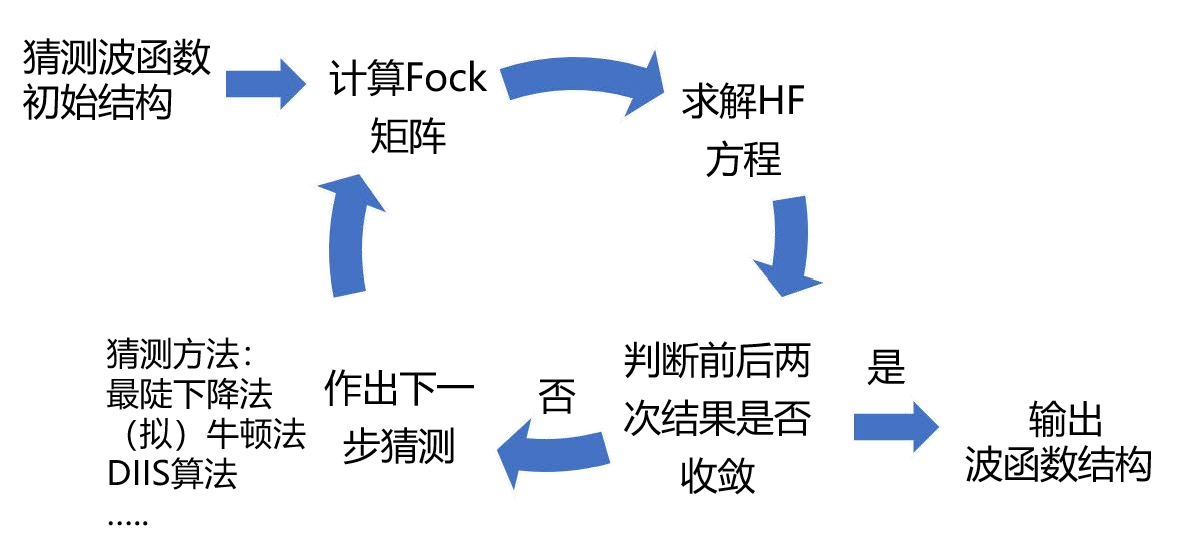
\includegraphics[width=0.7\textwidth]{figure/HF/HF_process.pdf}
\end{figure}
\end{frame}

%------------------------------------------------
%\subsection{SCF收敛难点}
%\begin{frame}
%\frametitle{SCF收敛难点}
%\begin{itemize}
%	\item 初猜选择的不合适,过于远离收敛区域;
%	\item 即使选择在收敛区域附近的初猜,迭代结果仍会逐渐偏离收敛点,即内禀性发散。\\
%	前线轨道能级密集体系极易出现内禀性发散现象。
%\end{itemize}
%
%\end{frame}

%------------------------------------------------

%\begin{frame}
%\frametitle{Multiple Columns}
%\begin{columns}[c] % The "c" option specifies centered vertical alignment while the "t" option is used for top vertical alignment

%\column{.45\textwidth} % Left column and width
%\textbf{Heading}
%\begin{enumerate}
%\item Statement
%\item Explanation
%\item Example
%\end{enumerate}

%\column{.5\textwidth} % Right column and width
%Lorem ipsum dolor sit amet, consectetur adipiscing elit. Integer lectus nisl, ultricies in feugiat rutrum, porttitor sit amet augue. Aliquam ut tortor mauris. Sed volutpat ante purus, quis accumsan dolor.

%\end{columns}
%\end{frame}

%------------------------------------------------
%\section{研究思路}
%------------------------------------------------
%\begin{frame}
%\frametitle{研究思路}
	%\begin{itemize}
	%	\item 迭代起始阶段着重于可以使能量快速下降\\
	%	EDIIS算法
	%	\item 过渡阶段\\
	%	DIIS算法与C$^2$DIIS算法
	%	\item 收敛区域附近着重于选取较小的迭代步长\\
	%	直接最小化算法,包括梯度下降法、拟牛顿法、RFO算法、RS-RFO算法与QN/DIIS算法
	%\end{itemize}
	
%	\begin{figure}[htbp]
%		\centering
%		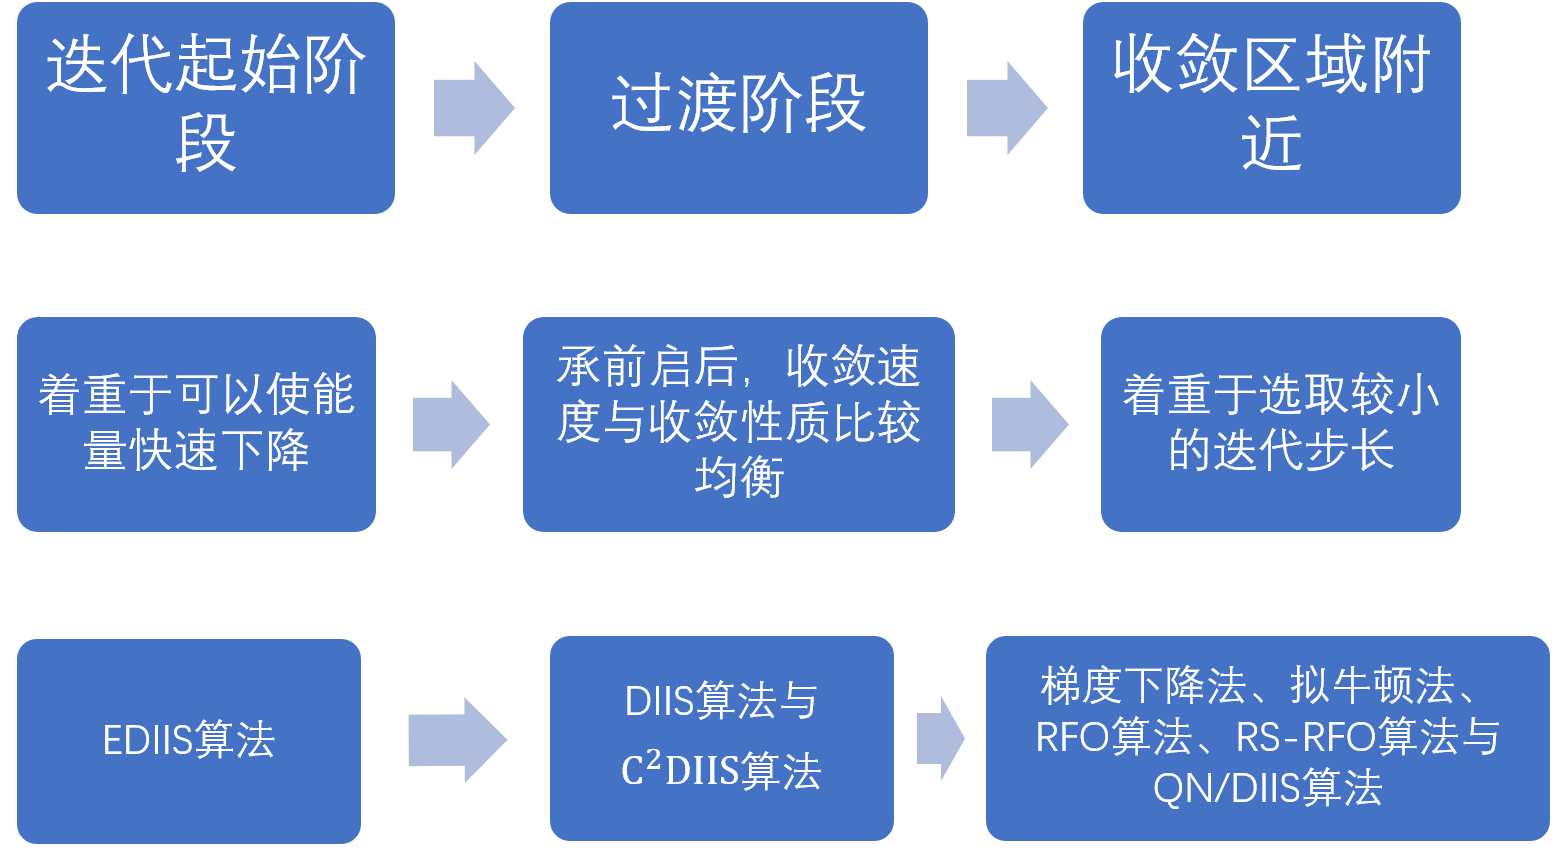
\includegraphics[width=0.9\textwidth]{figure/HF/idea.png}
%		\label{idea}
%	\end{figure}
%
%\end{frame}



%----------------------------------------------------------------------------------------
\section{研究内容}
%----------------------------------------------------------------------------------------


\begin{frame}
	\Huge{\centerline{研究内容}}
\end{frame}


%------------------------------------------------
\subsection{迭代起始阶段}
\begin{frame}
	\frametitle{EDIIS算法}
	每一步的输入为之前输出的内插值
	\begin{equation}
	D^{\text{in}} = \sum_{i=1}^{n} c_i D_i^{\text{out}}
	\end{equation}
	内插系数通过最小化能量泛函得到,即
	\begin{equation}
	\text{inf} \left \{f^{\text{EDIIS}} (c_1,c_2,..,c_n ),c_i \ge 0, \sum_{i=1}^n c_i =1\right \}
	\end{equation}
	能量泛函$f^{\text{EDIIS}}$的优化可以采用障碍法与能量面扫描的方法进行。
	%式中
	%\begin{equation}
	%f^{\text{EDIIS}} (c_1,c_2,..,c_n )=\sum_{i=1}^n c_i E(D_i) +\frac{1}{2}\sum_{i,j=1}^nc_i c_j \text{Tr}\left [(D_i-D_j )(F_i-F_j )\right]
	%\end{equation}
\end{frame}

%------------------------------------------------
\begin{frame}
	\frametitle{结果比较}
	二茂铁\\
	RHF/6-31G基组
	\begin{figure}[ht!]
		\centering
		\begin{minipage}{0.4\linewidth}
			\centering
			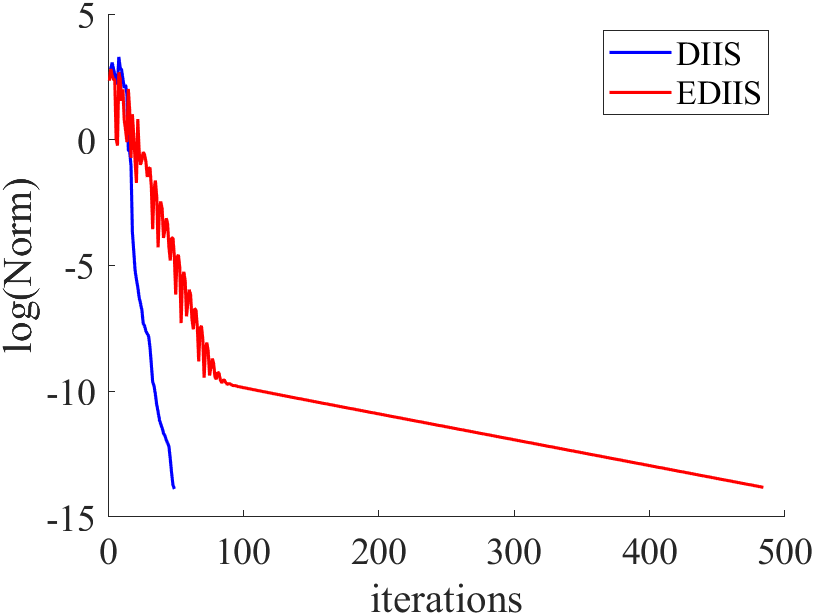
\includegraphics[height=3cm]{figure/ferrocene/logNorm2.png}
			\subcaption{梯度的模变化趋势}
			\label{fig:ferrocene:lognorm}
		\end{minipage}
		\begin{minipage}{0.4\linewidth}
			\centering
			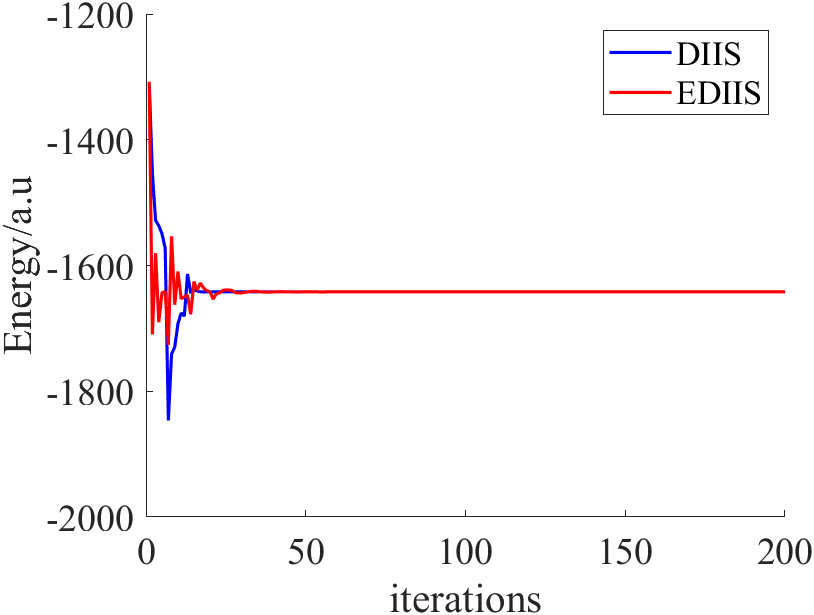
\includegraphics[height=3cm]{figure/ferrocene/E2.png}
			\subcaption{能量变化趋势}
			\label{fig:ferrocene:E}
		\end{minipage}
		\label{fig:ferrocene}
	\end{figure}
	\centerline{EDIIS算法可以有效降低收敛结果能量。}
\end{frame}

%------------------------------------------------
\begin{frame}
	\frametitle{EDIIS算法对收敛结果的影响}
	2,3-二乙基噻吩[3,4-B]吡嗪\\
	UHF/6-31G基组
	\begin{table}[htbp]
		%\centerline{2,3-二乙基噻吩[3,4-B]吡嗪的UHF计算结果。}
		\caption{2,3-二乙基噻吩[3,4-B]吡嗪的UHF计算结果。}\label{table:AA4}
		\setlength{\belowcaptionskip}{7pt}
		\centering
		\begin{tabular}{l l l}
			\toprule
			\textbf{算法} & \textbf{能量/(a·u)} & \textbf{迭代圈数}\\
			\midrule
			EDIIS(能量面扫描)         &-891.736841       &     497\\
			EDIIS(能量面扫描)+DIIS    &-891.701108      &     93\\
			EDIIS(障碍法)             & -891.734354      &      538\\
			EDIIS(障碍法)+DIIS        & -891.734354      &     90\\
			DIIS                      & -891.580787      &     57\\
			\bottomrule
		\end{tabular}
		\vspace{0.2cm}
	\end{table}
	\centerline{EDIIS算法的使用可以在初期快速降低收敛结果的能量。}
\end{frame}

%------------------------------------------------
\subsection{过渡阶段}
\begin{frame}
	\frametitle{DIIS算法与C$^2$DIIS算法}
	设定每次迭代的输入为
	\begin{equation}
		D^{\text{in}} = \sum_{i=1}^{n} c_i D_i^{\text{out}}
	\end{equation}
	同时设定对于$D_i^{\text{out}}$,其与最优解之间的误差为$e_i$,
	那么$D^{\text{in}}$与最优解之间的误差为
	\begin{equation}
		e^{*} = \sum_{i=1}^{n} c_i e_i
	\end{equation}
	通过最小化$e^{*}$的内积得到优化系数$\{c_i\}$,即最小化
	\begin{equation}
		\langle  e^{*} |  e^{*}  \rangle = \sum_{i,j=1}^{n} c_i c_j\langle  e_{i} |  e_{j}  \rangle
	\end{equation}
\end{frame}

%------------------------------------------------
\begin{frame}
	\frametitle{DIIS算法与C$^2$DIIS算法}

	\begin{itemize}
		\item DIIS算法要求$\sum_{i=1}^{n} c_i = 1$,则可通过求解线性方程组式\ref{DIIS}获得外推系数$\{c_i\}$
		\begin{equation}
		\begin{pmatrix}
		B_{11} & \ldots & B_{1n} & 1 \\
		\vdots & \ddots & \vdots & 1 \\
		B_{n1} & \ldots & B_{nn} & 1 \\
		1 & \cdots & 1 & 0
		\end{pmatrix}
		\begin{pmatrix}
		c_{1}\\
		\vdots\\
		c_{n}\\
		\lambda 
		\end{pmatrix}
		=
		\begin{pmatrix}
		0\\
		\vdots\\
		0\\
		1
		\end{pmatrix}
		\label{DIIS}
		\end{equation}
		\item C$^2$DIIS算法要求$\sum_{i=1}^{n} c_i^2 = 1$,则可通过求解本征方程式\ref{C2DIIS}获得外推系数$\{c_i\}$
		\begin{equation}
		\begin{pmatrix}
		B_{11} & \ldots & B_{1n} \\
		\vdots & \ddots & \vdots \\
		B_{n1} & \ldots & B_{nn} 
		\end{pmatrix}
		\begin{pmatrix}
		c_{1}\\
		\vdots\\
		c_{n}
		\end{pmatrix}
		=
		\lambda 
		\begin{pmatrix}
		c_{1}\\
		\vdots\\
		c_{n}
		\end{pmatrix}
		\label{C2DIIS}
		\end{equation}
	\end{itemize}
	上式中${B_{ij}} = \langle  e_{i} |  e_{j}  \rangle$
\end{frame}
%------------------------------------------------
\begin{frame}
	\frametitle{结果比较}
	一氧化碳\\
	UHF/6-31G基组
	\begin{figure}[ht!]
		\centering
		\begin{minipage}{0.4\linewidth}
			\centering
			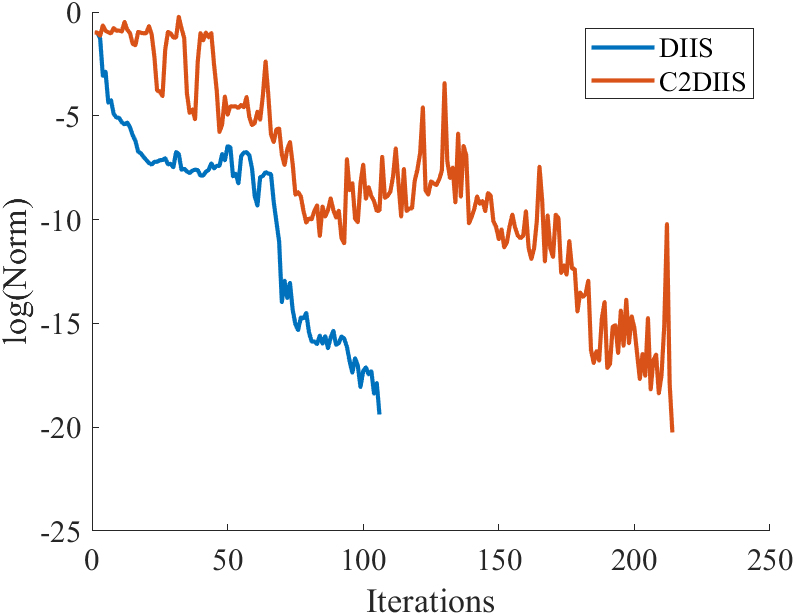
\includegraphics[height=3cm]{figure/co/LOG2.png}
			\subcaption{梯度的模变化趋势}
			\label{fig:co:lognorm}
		\end{minipage}
		\begin{minipage}{0.4\linewidth}
			\centering
			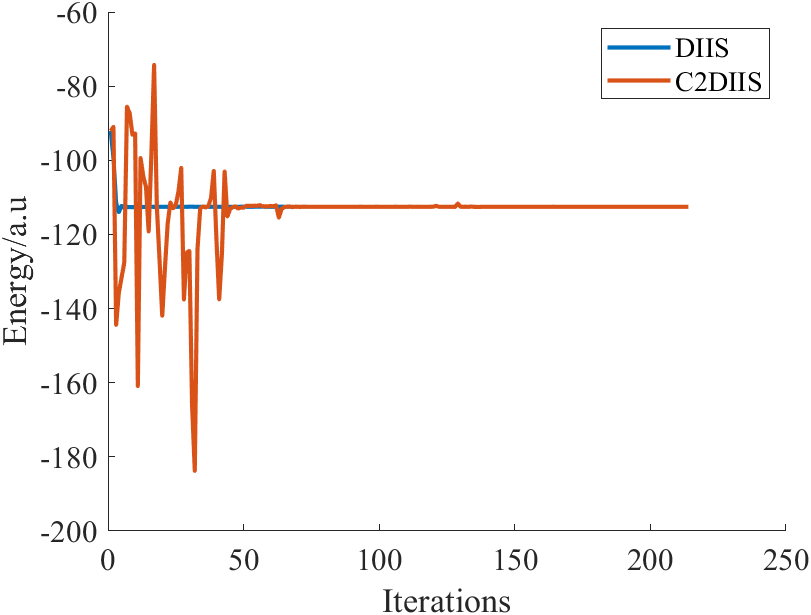
\includegraphics[height=3cm]{figure/co/E2.png}
			\subcaption{能量变化趋势}
			\label{fig:co:E}
		\end{minipage}
		\label{fig:co}
	\end{figure}
	\centerline{DIIS算法表现优异可以很快收敛,C$^2$DIIS算法性能逊于DIIS算法。}
\end{frame}


%------------------------------------------------
\subsection{收敛区域附近}
\begin{frame}
	\frametitle{直接最小化算法原理}
	\begin{itemize}
		\item
		HF方法的本质是在归一化条件下优化HF基态能量
		\begin{equation}
		E_{\text{Ground}}=\text{Min}\left \{ E_{\text{HF}}(C), C \in  \{C| C^TSC=I  \} \right \}
		\end{equation}
		可以直接优化参数求函数最小值
		
		\item 参数的选取\\
		每个满足条件的矩阵都可以表示为$C=C_0U$,$U=\text{exp}(-A)$,$C_0$表示起始系数矩阵\\
		我们将反厄米矩阵$A$的元素作为优化参数$\{x\}$进行优化
	\end{itemize}


	%$g_k$代表第$k$步的梯度向量\\
	%$H_k$代表第$k$步的Hessian矩阵\\
	%$B_k$代表第$k$步的Hessian矩阵的近似。
	
\end{frame}


%------------------------------------------------
\begin{frame}
	\frametitle{直接最小化算法}
	设优化的参数组成的向量为$p$,则
	\begin{itemize}
		\item 梯度下降法\qquad\quad
		$p_{k+1} = p_{k} -\alpha g_k$\\
		\item 牛顿法\qquad\qquad\quad
		$p_{k+1} = p_{k} -H^{-1} g_k$\\
		\item 拟牛顿法\qquad\qquad
		$p_{k+1} = p_{k} -B^{-1} g_k$\\
		\item 增强Hessian法\qquad
		$p_{k+1} = p_{k} -(H-\lambda I)^{-1} g_k$\\
		\item QN/DIIS算法\qquad\quad
		$p_{k+1} = \sum_{i=1}^{m} c_i p_{i} -\sum_{i=1}^{m} c_i H_k^{-1} g_i$
	\end{itemize}
	
	%$g_k$代表第$k$步的梯度向量\\
	%$H_k$代表第$k$步的Hessian矩阵\\
	%$B_k$代表第$k$步的Hessian矩阵的近似。
	
\end{frame}


%------------------------------------------------
\begin{frame}
	\frametitle{结果比较}
	苯分子\\
	UHF/6-31G基组
	\begin{figure}[ht!]
		\centering
		\begin{minipage}{0.4\linewidth}
			\centering
			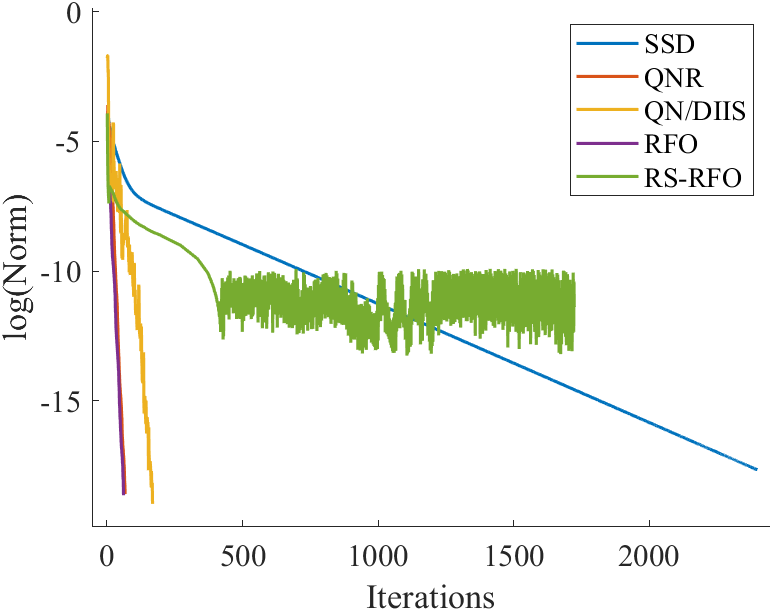
\includegraphics[height=3cm]{figure/benzene/NORM2.png}
			\subcaption{梯度的模变化趋势}
			\label{fig:benzene:lognorm}
		\end{minipage}
		\begin{minipage}{0.4\linewidth}
			\centering
			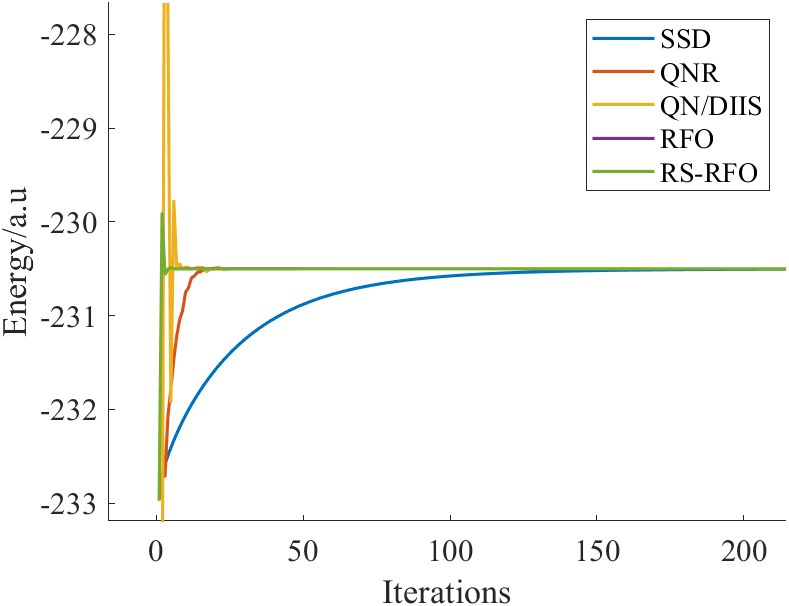
\includegraphics[height=3cm]{figure/benzene/E3.png}
			\subcaption{能量变化趋势}
			\label{fig:benzene:E1}
		\end{minipage}
	\end{figure}
	拟牛顿法与RFO算法的表现相对良好,SSD算法收敛速度较慢,QN/DIIS算法振荡明显,RS-RFO算法收敛失败。
\end{frame}
%------------------------------------------------
\subsection{组合算法}
\begin{frame}
	\frametitle{组合算法}
	在实际计算,单个算法的效果存在局限性,\\
	程序采用EDIIS算法与DIIS算法的组合,组合方式如下:
	
	\begin{equation}
		D^{in}=
		\begin{cases}
			D_{EDIIS}&\text{Norm}> 10^{-1},\\
			D_{DIIS}&\text{Norm}< 10^{-4},\\
			10\text{Norm} \times {D_{EDIIS}} + &\text{else}.\\
			\left( {1 - 10\text{Norm}} \right) \times {D_{EDIIS}}
		\end{cases}
	\end{equation}

	
\end{frame}


%------------------------------------------------
\begin{frame}
	\frametitle{结果比较}
	三氯化铁\\
	UHF/铁原子cc-pvdz基组,氯原子6-31G基组
	\begin{figure}[ht!]
		\centering
		\begin{minipage}{0.4\linewidth}
			\centering
			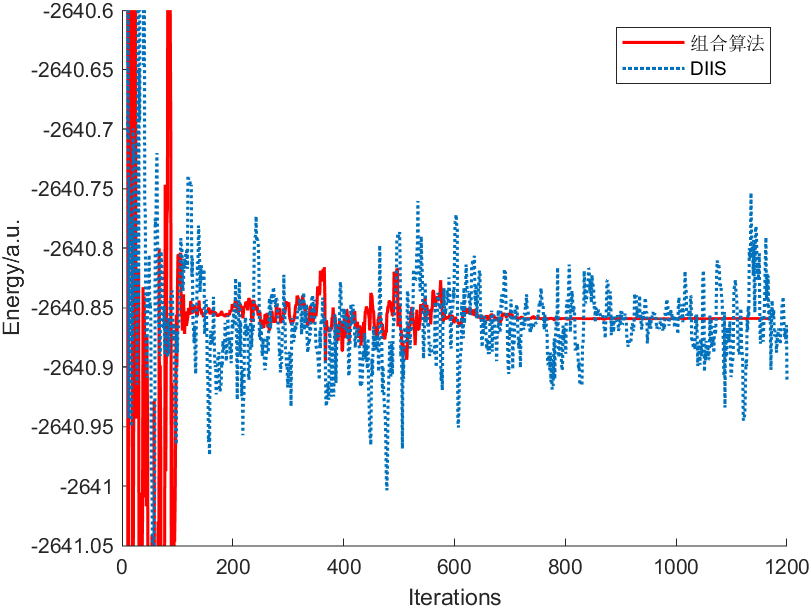
\includegraphics[height=3cm]{figure/FeCl3/E3.png}
			\subcaption{能量变化趋势}
			\label{fig:FeCl3:E}
		\end{minipage}
		\begin{minipage}{0.4\linewidth}
			\centering
			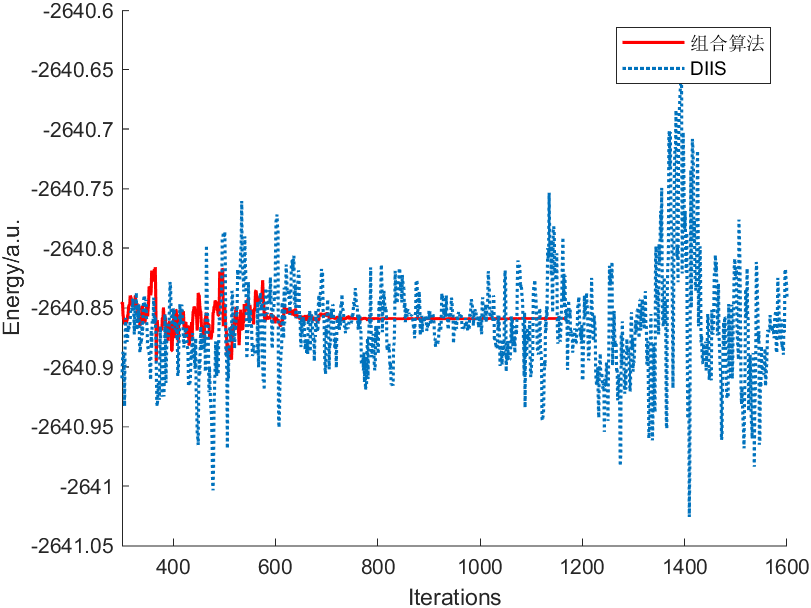
\includegraphics[height=3cm]{figure/FeCl3/FD3.png}
			\subcaption{收敛区域结果放大图}
			\label{fig:FeCl3:FD}
		\end{minipage}
	\end{figure}
	前期使用EDIIS算法可以有效抑制收敛区域的振荡,加速收敛,并降低收敛结果的能量。
\end{frame}

%----------------------------------------------------------------------------------------
\section{研究总结与展望}
%----------------------------------------------------------------------------------------

\begin{frame}
	\frametitle{研究总结与展望}
	总结
	\begin{itemize}
		\item[1)]
		 实现了DIIS及其衍生算法与QC算法,并对其进行测试;
		\item[2)] 
		 设计出一种组合算法,以计算出大多数体系。
	\end{itemize}
	
	展望
	\begin{itemize}
		\item [1)]
		EDIIS算法中参数优化算法需要进一步调整;
		\item [2)]
		各种算法之间的切换仍需进一步调整优化;
		\item [3)]
		进一步优化整体算法以计算含过渡金属的大分子体系。
	\end{itemize}
\end{frame}

%------------------------------------------------

%\begin{frame}
%	\frametitle{展望}
%	\begin{itemize}
%		\item [1)]
%		EDIIS算法中参数优化算法需要进一步调整;
%		\item [2)]
%		各种算法之间的切换仍需进一步调整优化;
%		\item [3)]
%		进一步优化整体算法以计算含过渡金属的大分子体系。
%	\end{itemize}
%	
%\end{frame}

%------------------------------------------------
\begin{frame}
	\frametitle{致谢}
	感谢马海波老师的悉心指导,在论文完成的过程中给了我莫大帮助,这个课题也让我对量子化学有了更进一步的认识。\\
	感谢谢兆轩师兄与李健浩师兄在我完成论文期间,给我的一系列意见与指导,帮我解答一系列困惑。\\
	也感谢实验室其他师兄师姐在我完成毕设期间,给我提供的帮助。
\end{frame}

%------------------------------------------------

\begin{frame}
	\Huge{\centerline{谢谢!}}
	\Huge{\centerline{敬请各位老师}}
	\Huge{\centerline{批评指正!}}
\end{frame}

%----------------------------------------------------------------------------------------
\end{document} 